%% Dit is de domeinanalyse: Composite Objects %%
%% Freek 26 september: Een derde domeinanalyse zou kunnen gaan over hoe om te
%% gaan met Composite objects (bijv. hoe grafisch weer te geven, hoe op te
%% slaan in de data structuur)

\documentclass[a4paper,11pt,final]{article}

\usepackage[english]{babel}
\usepackage{graphicx}
\usepackage{hyperref}
\hypersetup{ colorlinks = true, citecolor = blue,linkcolor = blue }
\usepackage[a4paper]{geometry}
\usepackage{titlesec}% added to change section headers, see newcommand definition.


\bibliographystyle{alpha}

		

\begin{document}
\selectlanguage{english}
\begin{titlepage}
	\vspace*{\fill}
	\begin{center}
		\textsc{\large WickedXmas Domain Analysis}\\[0.5cm]
		\textsc{\huge Composite Objects}\\[0.5cm]
		\textsc{Stefan Versluys}\\ \textsc{\scriptsize 19/10/2014}\\[2.0cm]
		
\includegraphics[width=0.25\textwidth]{wXm}
	\end{center}
	\vspace*{\fill}
\end{titlepage}


\tableofcontents

\newpage

\section{Introduction}
\paragraph{}
This domain analysis concerns composite objects,
along with primitive objects this kind of objects can be used to design xMAS
models with the WickedXmas tool. In fact composite objects are xMAS models
itself but left open with connection points, parameterizable and allow reuse.
The benefits of composite objects are those of reusability, it makes complex
things look simple and maintainable, it preserves correctness.

When designing an xMAS model in WickedXmas, the designer can make use of
composite objects similar as he or she does with primitive objects. Because
composite objects are xMAS models these can be edited just as any other kind
of xMAS model except that there are connection points as mentioned before.

\paragraph{}
In the next section you'll find a briefly description of the WickedXmas tool,
so you'll get an idea of how combinatorial objects are managed and (re)used.
After that there's a description of the properties from primitive objects
followed by these of composite objects.
How models are stored as a  persistent data structures will be discussed in
the JSON section.

To finalise you'll find a domain example out of an other kind of industry but
who had the same reason to build a graphical design tool and with a lot of
simularities.
Especially the management and facilities of reusable objects is an 
interesting topic which can inspire future designers or users of the
WickedXmas tool.

\newpage
\section{WickedXmas}
In this section we'll describe the WickedXmas tool briefly, the tool is used
to create, edit, view or verify xMAS models. Secondly I will show how
composite objects are created and used in this tool.
WickedXmas saves models as json formatted files which have "wck" as
extension. The same holds for composite objects with some minor
differences. Models can be made of primitive objects and composite objects,
to visualise models, objects have graphical properties along with some
specific properties. 
This document only concerns the properties necessary to represent an
xMAS model so it can be visualised,edited, stored and exchanged with
the verification interface.

\begin{figure}[here]
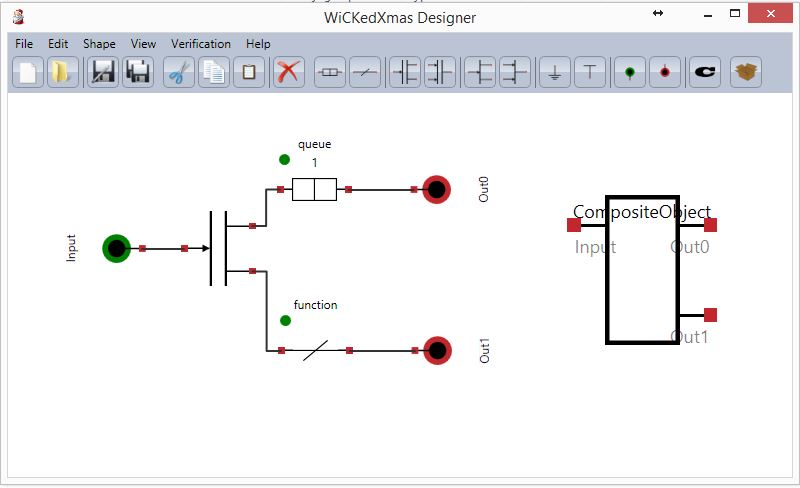
\includegraphics[width=1.0\textwidth]{wxmCO}
\caption{WickedXmas Tool and Composite objects}
\label{fig:wxmCO}
\end{figure}
Figure~\ref{fig:wxmCO} shows us the WickedXmas tool visualising the contents
of "CompositeObject.wck". At the left side we see that this is a composite
object because of the connection points. At the right side you see how this 
composite object is visualised when it is reused.

In the toolbar you can see several buttons, eight of these are used to draw
primitive objects which are discussed in the next section. You can recognise
these by the pictogram in the button. Then two other buttons are used to
draw an input or output connection point followed by a button with a big "C"
in it which is used to add a composite object for reuse.
The button with the open box image opens the packet configuration
window where a user can add fields with their ranges. These fields can be
used into the function property of the objects used in the model.


\newpage
\section{Primitive objects}
Primitive objects are the base of xMAS models and determine the underlying structures.
Secondly, when using objects to create a model, there are a lot of similarities between
composite and primitive objects. With this knowledge we can say that
primitive objects need some explanation as far as these are concerned with
composite objects and modelling using the WickedXmas tool.

The xMAS language has only eight primitive objects,
each object has a visual representation and one or more properties which can be
changed. Some of these properties requires a valid value otherwise a
visual marker, shown as a dot as part of the object, will lit up red instead of
green. Finally all objects have one or more ports and can be of input or output
type. The graphical representation of a port is a red filled square. 
To form a valid channel, each port must be wired to exactly to one
opposite porttype of an other object.

\paragraph{Common properties:}
\begin{itemize}
\item Label: A string which identifies the object.
\item Position: x and y-coordinates where the object is drawn on screen.
\item Orientation: A value that represents the direction in which the object is drawn on screen.
\end{itemize}

\subsection{Queue}
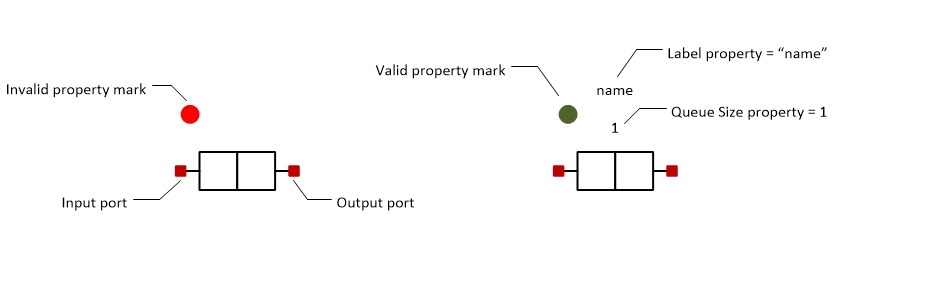
\includegraphics[width=1.0\textwidth]{queue}
The queue object its valid marker becomes green when the size property is a natural number $>$ 0. 
The queue also have a "state" property to show the verification result. 
\paragraph{Specific properties:}
\begin{itemize}
\item Size: A positive integer which represents the storage size of a queue.
\item State: Used to visualise the verification result.
\end{itemize}

\subsection{Function}

\includegraphics[width=1.0\textwidth]{function}
\paragraph{Specific properties:}
\begin{itemize}
\item Function f: is a subset of the C language, an integer which represents the packet is available through variable 'header'.
The valid marker becomes green if the  string value of the "Function f" property is not empty.

Example: ret=0;

Available operators:
\begin{itemize}
\item math operators $+,-,*,/,\%$
\item logical operators $\&\&,||,!$
\item equality operators $==,<=,>=,<,>$
\end{itemize}
\end{itemize}


\subsection{Fork}
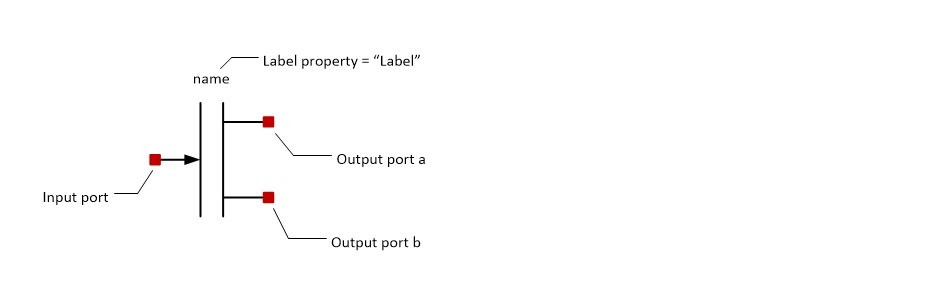
\includegraphics[width=1.0\textwidth]{fork}
A fork has no specific properties.


\subsection{Join}
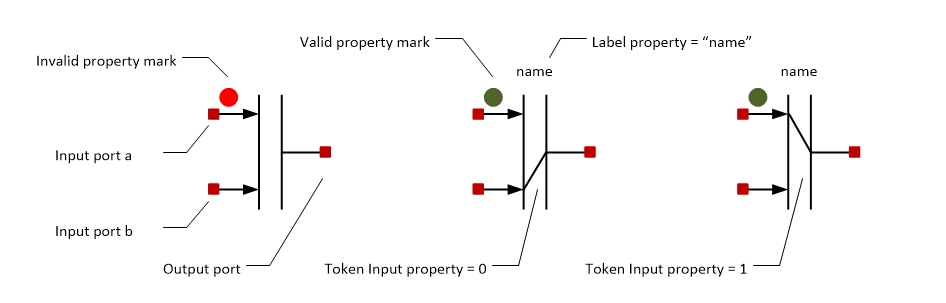
\includegraphics[width=1.0\textwidth]{join}
The join object its valid marker becomes green if the "token" property is set. Depending on the "token" property the visualisation of the object will change.
\paragraph{Specific properties:}
\begin{itemize}
\item Token Input: "0" select input 2 while "1" selects input 1
\end{itemize}


\subsection{Switch}
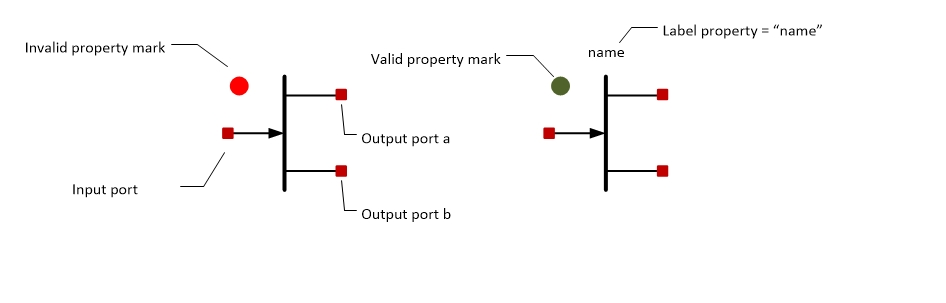
\includegraphics[width=1.0\textwidth]{switch}
\paragraph{Specific properties:}
\begin{itemize}
\item "Function s" is a subset of the C language, an integer which represents the packet is available through variable 'header'.
The valid marker becomes green if the  string value of the "Function s" property is not empty.

Example: return header == 0;

Available operators:
\begin{itemize}
\item math operators $+,-,*,/,\%$
\item logical operators $\&\&,||,!$
\item equality operators $==,<=,>=,<,>$
\end{itemize}
\end{itemize}


\subsection{Merge}
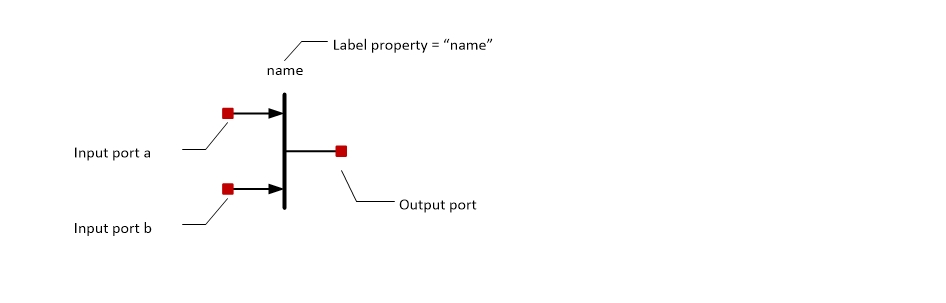
\includegraphics[width=1.0\textwidth]{merge}
A merge has no specific properties.

\subsection{Sink}
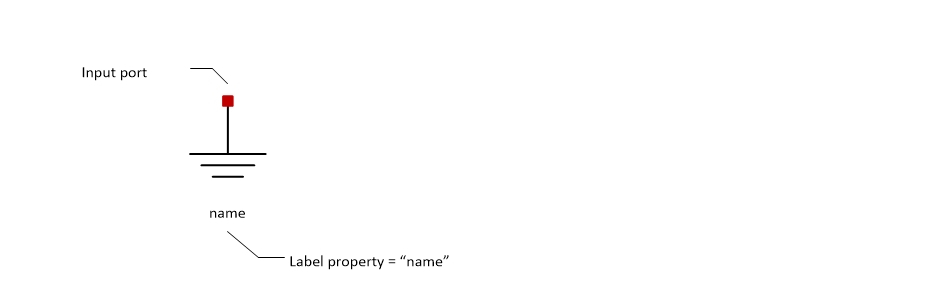
\includegraphics[width=1.0\textwidth]{sink}
A sink has no specific properties.

\subsection{Source}

\includegraphics[width=1.0\textwidth]{source}
\paragraph{Specific properties:}
\begin{itemize}
\item "Function e" insert types of packets injected at this source. The domain of all packets is available through PacketDomain.
The valid marker becomes green if the  string value of the "Function e" property is not empty.

Example: \{p in PacketDomain $|$ p $<$ 100\}
\end{itemize}


\section{Composite objects}
Because a composite object is an open network, WickedXmas provides two
additional objects to create connection points, which are in fact the resulting
ports of the composite object itself. This is to distinguish between a
dangling port and one that will be connected later when reusing the
composite object.

There are two kinds of connection points, the input type and the output type.
In figure~\ref{fig:CompObj} at the left you can find the graphical
representation of these objects. The properties of connection points are
the same as those for primitives and do not have any specific properties.
In the center of figure~\ref{fig:CompObj} a simple example of a
composite object being opened e.g. for editing. It is saved as file MyQ.wck
and can be reused into a larger model as shown right in figure ~\ref{fig:CompObj}.

As you can see the filename of a composite object is placed in its
body when reuse. The size of the body will be adjusted by the number
of ports, input ports left and output ports at the right.


\begin{figure}[here]
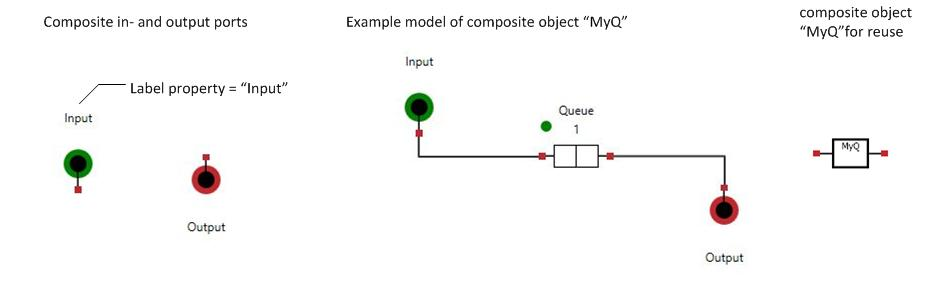
\includegraphics[width=1.0\textwidth]{CompObj}
\caption{Composite object}
\label{fig:CompObj}
\end{figure}


\newpage
\section{JSON}
ToDo : to be completed
\subsection{Hierarchical structure}
\subsection{Flat structure}

\newpage
\section{Similar domain examples}
ToDo : example of how a similar product manages re-usable components

\newpage
\section{Dictionary}
\begin{itemize}
	\item \textbf{WickedXmas}: Name ofthe tool used to design and analyse xMAS models.
	\item \textbf{xMAS model}:
	A model based on Intel's xMAS or e\underline{x}ecutable \underline{M}icro\underline{A}rchitectural \underline{S}pecification,
	which is ahigh level design language for communication fabrics.
	\item \textbf{Primitive Object}: The xMAS language consist of eight primitive objects which are used to create xMAS models.
	Primitive objects are hard coded.
	\item \textbf{Composite Object}: A composite object which can be made of primitives and composite objects.
	It is also known as a open xMAS model, macro or combinatorial object.
	\item \textbf{Channel}: A connection between an input and output port.
	\item \textbf{Port}: Each object has one or more ports to create a channel, there are initiator and target ports.
	\item \textbf{Initiator}: An output port.
	\item \textbf{Target}: An input port.
	\item \textbf{Open xMAS network}: see Composite object.
	\item \textbf{Macro or macro block}: see Composite object.
	\item \textbf{Combinatorial object}: see Composite object.
	\item \textbf{Connection point}: Object to create a port for a composite object.
	\item \textbf{Configuration}: Represents the current state of a model which means the occupation of queues.
	\item \textbf{wck}: File extension of an xMAS model and contains hierarchical structured JSON.
	\item \textbf{JSON}: \underline{J}avascript \underline{O}bject \underline{N}otation is a readable data file format comparable to XML.
	\item \textbf{fjson}: File extension of an xMAS model and contains flat structured JSON.
	\item \textbf{Message type}: Thereresponse or request
\end{itemize}

\end{document}